\begin{frame}{How to measure 3D diffraction patterns at SixS ?}
    \begin{columns}
        \column[T]{0.45\textwidth}
        \begin{figure}
            \centering
            \begin{tikzpicture}
                \node (image) [anchor=south west, inner sep=0pt] {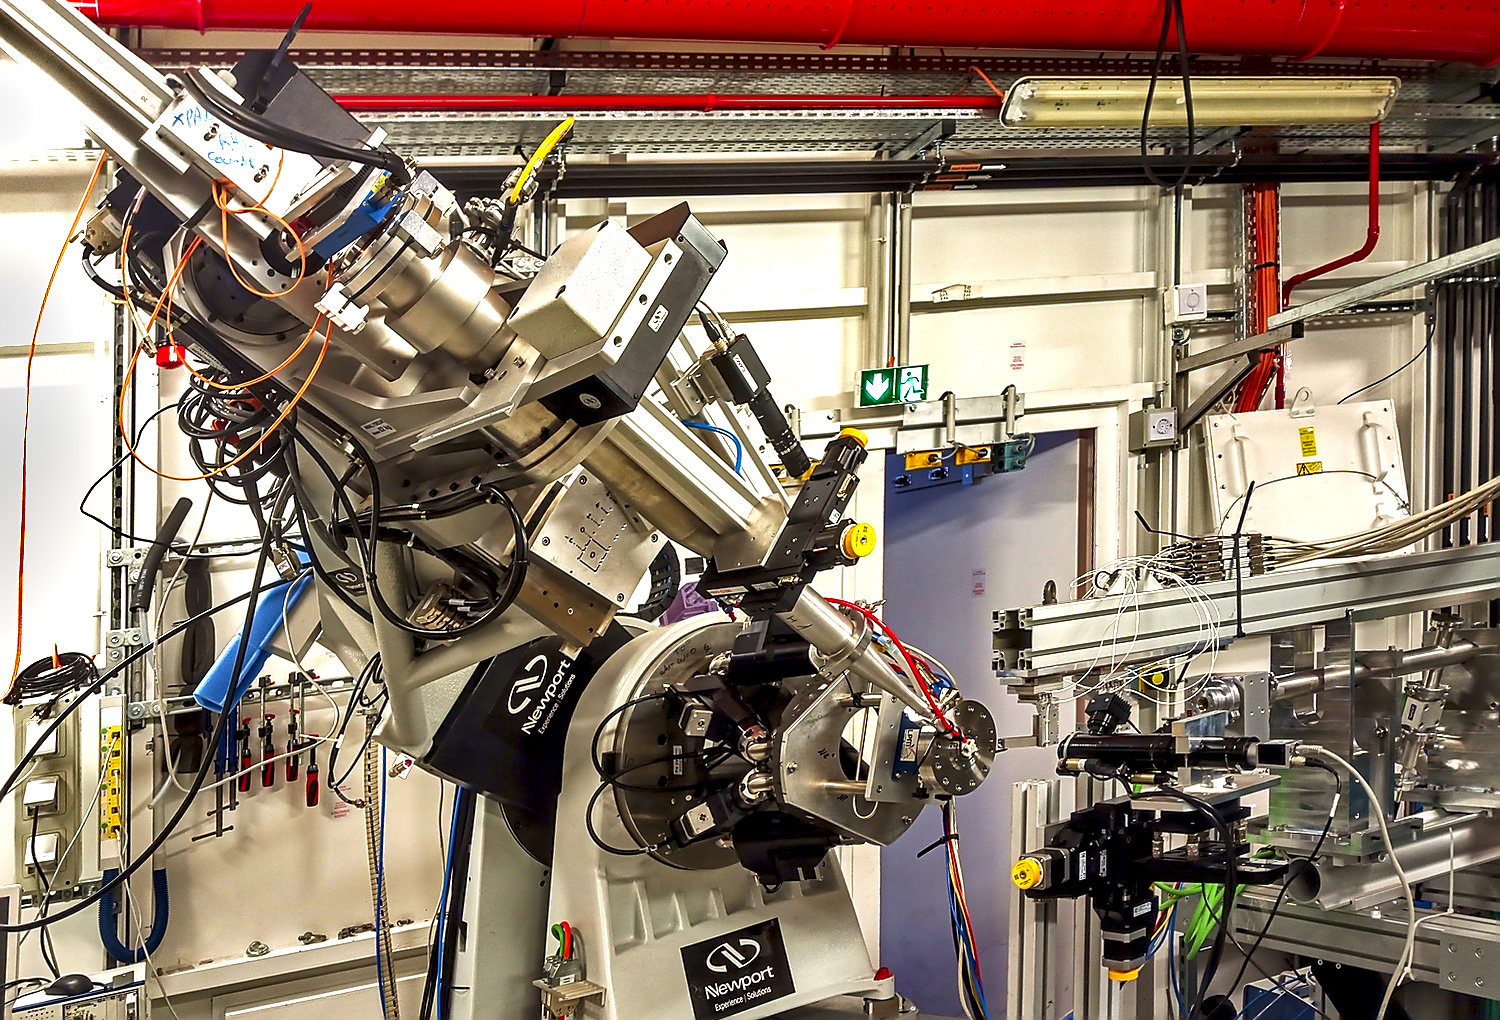
\includegraphics[trim=0 30 100 20, clip, width=\textwidth]{Figures/sixs/MED.jpg}};
                \begin{scope}[x={(image.south east)}, y={(image.north west)}]
                    \node [fill=white,rounded corners=2pt,inner sep=1pt] at (0.7,0.2) {Sample};
                    \node [fill=white,rounded corners=2pt,inner sep=1pt] at (0.35,0.7) {Detector};
                \end{scope}
            \end{tikzpicture}
            \caption{Multi Environment Diffractometer (MED), experimental end station at SixS}
            \label{fig:MED_3D}
        \end{figure}
        
        \vspace{-0.4cm}
        
        \begin{gather*}
            I(\vec{q}_{hkl}) \propto ||F(\vec{q}_{hkl})||^2\\
            F(\vec{q}_{hkl}) = \sum_j^N f_j (\vec{q}_{hkl}) \exp^{i(\vec{q}_{hkl}.\vec{u}(\vec{r}))}
        \end{gather*}

        \column[T]{0.45\textwidth}
        
    \end{columns}
    
\end{frame}


\begin{frame}{How to measure 3D diffraction patterns at SixS ?}
    \begin{columns}
        \column[T]{0.45\textwidth}
        \begin{figure}
            \centering
            \begin{tikzpicture}
                \node (image) [anchor=south west, inner sep=0pt] {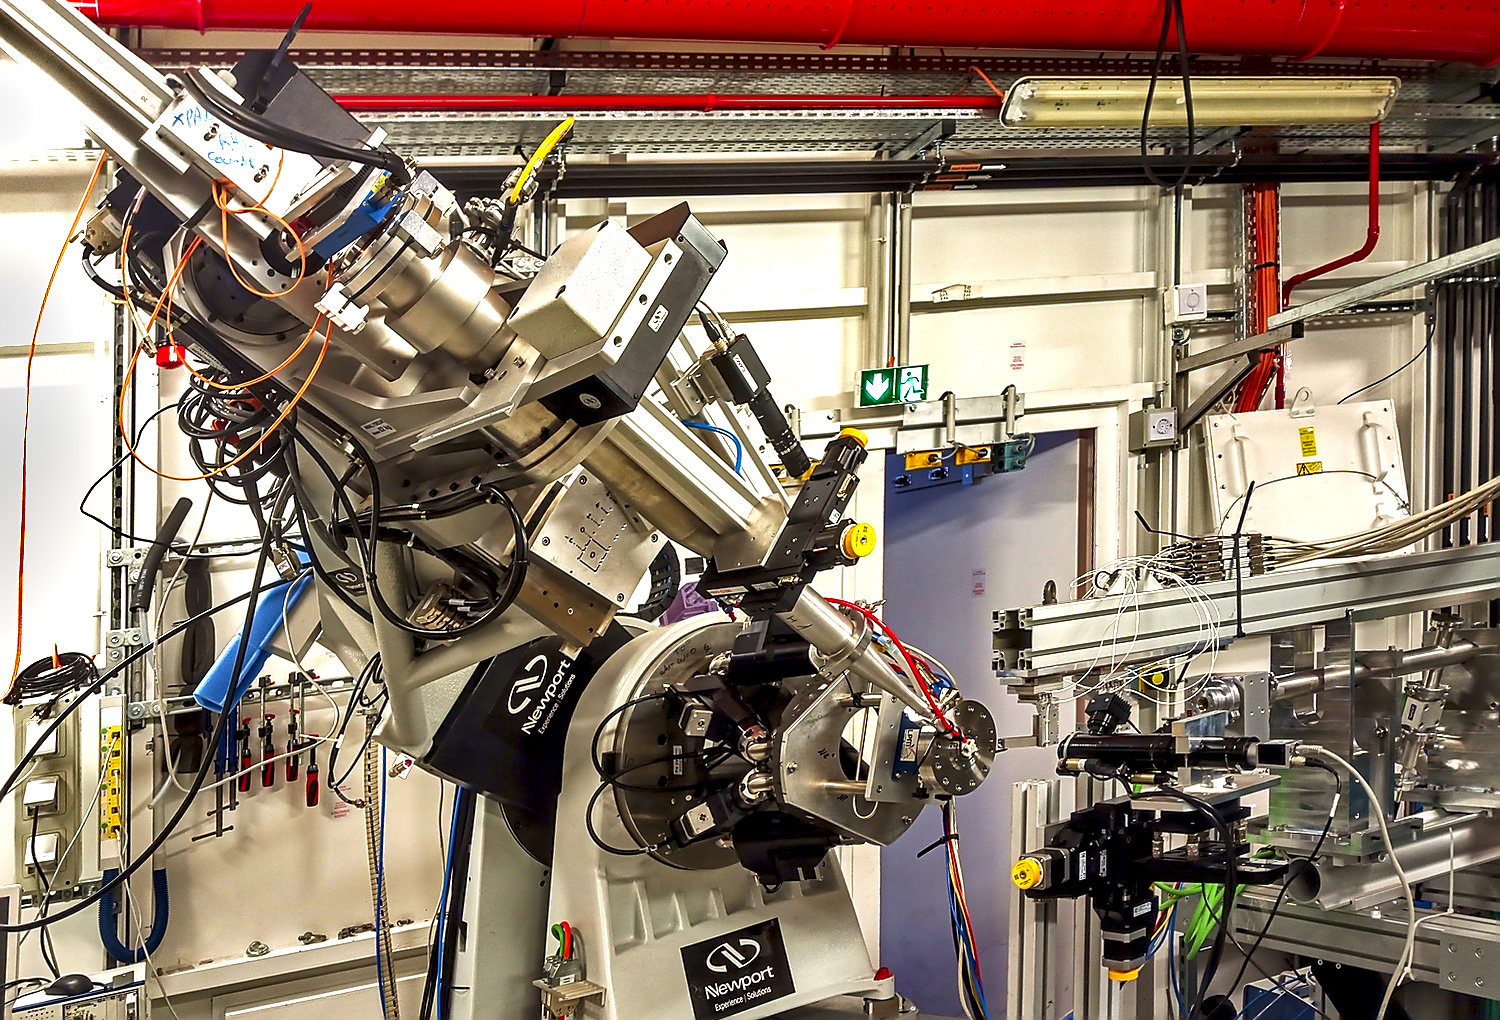
\includegraphics[trim=0 30 100 20, clip, width=\textwidth]{Figures/sixs/MED.jpg}};
                \begin{scope}[x={(image.south east)}, y={(image.north west)}]
                    \node [fill=white,rounded corners=2pt,inner sep=1pt] at (0.7,0.2) {Sample};
                    \node [fill=white,rounded corners=2pt,inner sep=1pt] at (0.35,0.7) {Detector};
                \end{scope}
            \end{tikzpicture}
            \caption{Multi Environment Diffractometer (MED), experimental end station at SixS}
        \end{figure}
        
        \vspace{-0.4cm}
        
        \begin{gather*}
            I(\vec{q}_{hkl}) \propto ||F(\vec{q}_{hkl})||^2\\
            F(\vec{q}_{hkl}) = \sum_j^N f_j (\vec{q}_{hkl}) \exp^{i(\vec{q}_{hkl}.\vec{u}(\vec{r}))}
        \end{gather*}

        \column[T]{0.45\textwidth}
        
        \begin{figure}
            \centering
            \animategraphics[trim=200 0 200 0, autoplay,loop, clip, width=0.9\textwidth]{5}{Figures/bcdi_data/3D_DP/DP_white_}{1}{20}
            \caption{Coherent fringes visible in multiple directions in 3D diffraction pattern}
        \end{figure}
    \end{columns}
    
\end{frame}